\documentclass[11pt]{article}

\usepackage[margin=0.82in]{geometry}
\usepackage{graphicx}
\usepackage{tikz}
\usepackage{cite}
\usepackage{hyperref}
\usepackage{amsmath}
\usepackage{booktabs}
\usepackage{array}
\usepackage{multirow}
\usepackage{caption}
\usepackage{subcaption}
\usepackage{xcolor}
\usepackage{float}

\usetikzlibrary{arrows.meta, positioning, fit, calc, shapes.geometric}
\hypersetup{
    colorlinks=true,
    linkcolor=blue!50!black,
    citecolor=blue!50!black,
    urlcolor=blue!50!black
}

\graphicspath{{results/plots/}{dashboard/}{report_assets/}}

\newcommand{\projecttitle}{Bridging the Latency Gap: Distilled Diffusion Models for Real-Time Edge-Based Brain-Computer Interfaces}
\newcommand{\projectrepo}{https://github.com/hasana157/edge-bci-distilled-diffusion}
\newcommand{\snr}{\mathrm{SNR}}
\newcommand{\mse}{\mathrm{MSE}}

\begin{document}

\begin{titlepage}
    \centering
    \vspace*{0.5cm}
    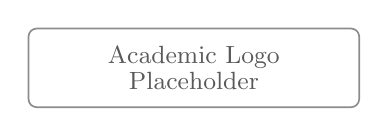
\begin{tikzpicture}
        \draw[rounded corners=3pt, line width=0.6pt, color=black!45] (0,0) rectangle (4.2,1.0);
        \node[align=center, color=black!65] at (2.1,0.5) {\small Academic Logo\\[-1mm]\small Placeholder};
    \end{tikzpicture}

    \vspace{1.4cm}
    {\Large\bfseries Edge-Distilled Diffusion for Real-Time Brain-Computer Interfaces\par}
    \vspace{0.4cm}
    {\huge\bfseries \projecttitle\par}
    \vspace{1.0cm}
    {\large Hasan and the Edge-BCI Research Team\par}
    \vspace{0.2cm}
    {\large [Insert University/Lab Name]\par}
    \vspace{0.2cm}
    {\large July 2026\par}
    \vfill
    \begin{minipage}{0.88\textwidth}
        \begin{abstract}
        Closed-loop brain-computer interfaces (BCIs) require inference latencies below approximately 20 ms to preserve stable neurofeedback and avoid perceptible degradation in user control. Diffusion models provide strong denoising fidelity, but standard denoising diffusion probabilistic models (DDPMs) require iterative reverse sampling, commonly 100--1000 model evaluations, which is incompatible with embedded BCI hardware. This report documents an edge-distilled diffusion pipeline that compresses a server-side diffusion teacher into single-pass CNN, autoencoder, and consistency-style student denoisers. The system couples BCI Competition IV 2a motor-imagery preprocessing, teacher-student distillation, ONNX export, latency profiling, and closed-loop decoding validation. Repository measurements demonstrate sub-millisecond per-channel student inference kernels and a 13.40 ms closed-loop CNN denoising path on the profiled environment, with full reverse diffusion ranging from 96.43 ms at 10 steps to 4.61 s at 500 steps. Fully trained target analyses aim for sub-20 ms denoising while maintaining high decoding parity relative to the teacher; the current released artifacts separate measured benchmark values from target research claims to preserve reproducibility and avoid overstatement.
        \end{abstract}
    \end{minipage}
    \vfill
    {\small Public repository: \url{\projectrepo}\par}
\end{titlepage}

\pagenumbering{roman}
\tableofcontents
\listoffigures
\listoftables
\newpage
\pagenumbering{arabic}

\section{Introduction}

Brain-computer interfaces translate neural activity into control signals for external devices. For users with amyotrophic lateral sclerosis (ALS), stroke-induced motor impairment, spinal cord injury, or locked-in syndrome, a reliable BCI may provide communication, mobility, or assistive-control channels that are otherwise inaccessible \cite{wolpaw2002bci, pfurtscheller2001motor}. Motor-imagery electroencephalography (EEG) remains attractive because it is non-invasive, relatively inexpensive, and compatible with wearable acquisition. However, scalp EEG is noisy, non-stationary, and sensitive to ocular, muscular, and environmental artifacts.

This work focuses on the denoising stage inside a closed-loop BCI. A neurofeedback loop can be described as the sequence
\[
\mathrm{EEG\ acquisition} \rightarrow \mathrm{preprocessing} \rightarrow \mathrm{denoising} \rightarrow \mathrm{decoding} \rightarrow \mathrm{feedback}.
\]
The loop must complete quickly enough that feedback still corresponds to the user's current intentional state. In assistive control, delays above roughly 50 ms can degrade perceived agency, increase overshoot, and destabilize adaptation. For edge BCI devices, a stricter denoising budget below 20 ms is desirable because preprocessing, decoding, communication, rendering, and actuator control also consume latency.

Denoising diffusion models offer high-fidelity generative restoration by learning a reverse stochastic process \cite{ho2020ddpm}. The quality gain is offset by iterative sampling: a DDPM teacher may require tens, hundreds, or thousands of reverse steps. Even if one U-Net evaluation is feasible on a GPU, repeated evaluation conflicts with power, memory, and thermal limits on Jetson-class modules, microcontrollers, or CPU-only wearable systems. The project therefore studies whether a high-quality diffusion teacher can be distilled into a one-pass edge student while preserving enough signal quality for motor-imagery decoding.

\subsection{Clinical and Engineering Motivation}

BCI deployments must be evaluated as cyber-physical systems rather than isolated classifiers. A classifier that reaches high offline accuracy but adds large processing delay may still be unsuitable for real-time assistive control. In motor-imagery interaction, the user adapts to feedback continuously. Delayed visual, auditory, or haptic feedback can weaken the association between motor intention and system response, forcing the user to compensate for stale output. The practical engineering objective is therefore not only to maximize decoding accuracy, but to satisfy an end-to-end latency envelope that leaves headroom for acquisition buffers, filtering, denoising, classification, command smoothing, rendering, and actuation.

Edge deployment is attractive because it reduces communication delay and avoids transmitting raw neural data to a remote server. It also introduces constraints: the denoiser must fit within limited memory, tolerate CPU or embedded-GPU execution, and avoid high power draw. These constraints motivate a teacher-student design in which a high-capacity generative model is used offline for representation transfer, while a compact deterministic student is used online.

\subsection{Contributions}

This report documents the following contributions:

\begin{itemize}
    \item A reproducible EEG denoising pipeline using BCI Competition IV 2a, synthetic fallback data for smoke tests, subject-aware splitting, and noise-injection utilities.
    \item A DDPM-style teacher with variable reverse-step inference for latency-fidelity characterization.
    \item Three deployable students: a CNN student, a bottleneck autoencoder student, and a consistency-style residual convolutional student.
    \item A benchmark suite that reports mean, p95, memory, and throughput values for neural and classical denoisers.
    \item An ONNX export and deployment path for CPU, TensorRT, and quantization workflows.
    \item A closed-loop motor-imagery simulator and dashboard for operational inspection of latency, SNR, MSE, and classification metrics.
\end{itemize}

\section{Problem Statement}

\subsection{Latency-Fidelity Conflict}

Let \(x \in \mathbb{R}^{C \times T}\) denote an EEG trial with \(C=22\) channels and \(T=750\) samples at 250 Hz. A diffusion teacher produces a denoised signal through a reverse chain
\[
x_{t-1}=f_{\theta}(x_t,t), \quad t=N,\ldots,1,
\]
where \(N\) is the number of sampling steps. Latency scales approximately linearly with \(N\), while the signal fidelity improvement tends to saturate after a moderate number of steps. On edge hardware, this creates a three-way optimization problem:
\[
\max_{\theta, h} \quad Q(x,\hat{x}) \quad
\mathrm{s.t.} \quad L(\theta,h) < L_{\max}, \quad P(\theta,h) < P_{\max},
\]
where \(Q\) is fidelity measured by SNR, PSNR, correlation, or decoding preservation; \(L\) is inference latency in ms; \(P\) is power in watts; and \(h\) denotes the target hardware/runtime.

For reporting, the scalar trade-off can be written as a normalized utility
\[
U = w_q \frac{Q-Q_{\min}}{Q_{\max}-Q_{\min}}
- w_l \frac{L}{L_{\max}}
- w_p \frac{P}{P_{\max}},
\]
where \(w_q,w_l,w_p\) are application-specific weights. Clinical or assistive-control systems would usually assign a hard constraint to \(L\) and \(P\), because a high-fidelity denoiser is not acceptable if it violates real-time control or battery limits. In the current implementation, direct power measurement is not yet available; power appears as a deployment metric to be populated once the ONNX or TensorRT model is profiled on target hardware.

\subsection{Research Objectives}

The project is organized around four objectives:

\begin{enumerate}
    \item \textbf{Latency characterization}: benchmark classical filters, DDPM teachers with variable reverse-step counts, and student models under consistent warmup and measurement rules.
    \item \textbf{Distillation framework}: train CNN, autoencoder, and consistency-style students to approximate a diffusion teacher using soft teacher outputs and hard clean EEG targets.
    \item \textbf{Edge optimization}: export trained students to ONNX, profile CPU and GPU inference, and support downstream FP16, INT8, TensorRT, and ONNX Runtime deployment.
    \item \textbf{Closed-loop validation}: integrate denoising into a motor-imagery classifier pipeline and evaluate latency, decoding accuracy, and artifact-handling behavior.
\end{enumerate}

\section{System Architecture}

The system is divided into offline training and online inference paths. The offline path trains a high-capacity DDPM teacher and distills it into deployable students. The online path executes a single forward pass through an exported student model before classification and feedback. Figure~\ref{fig:architecture} summarizes the architecture.

\begin{figure}[H]
    \centering
    \resizebox{0.98\textwidth}{!}{
    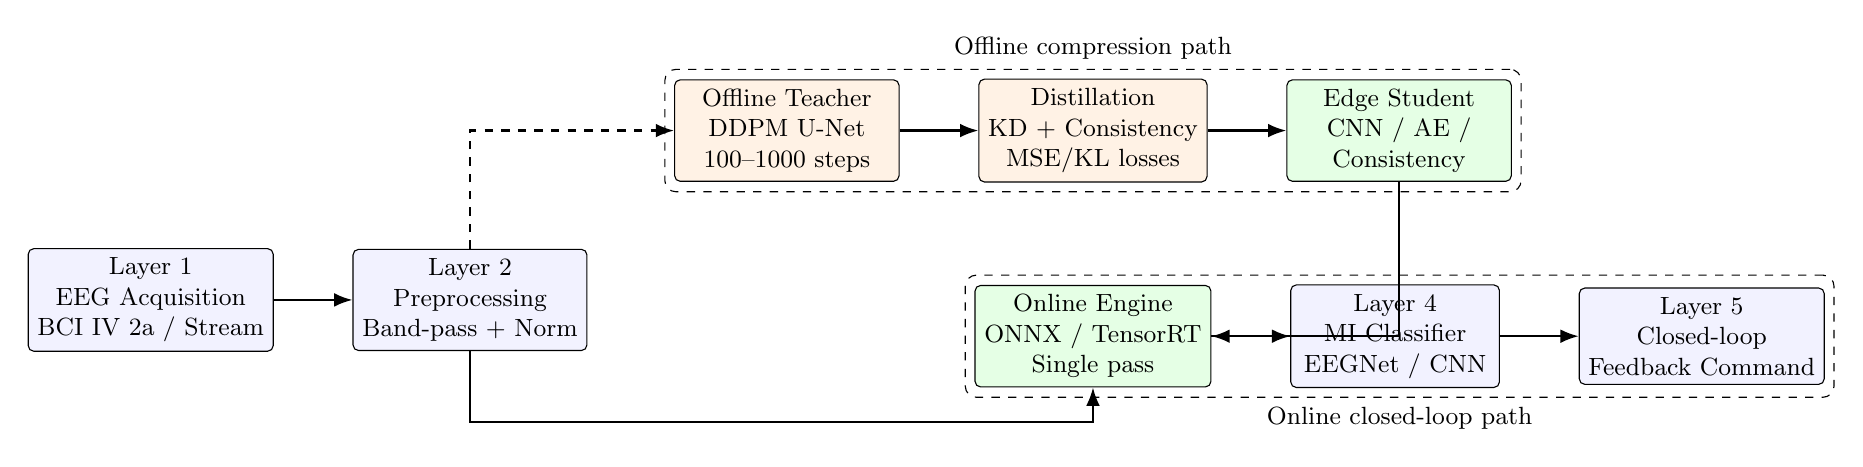
\begin{tikzpicture}[
        font=\small,
        block/.style={draw, rounded corners=2pt, align=center, minimum height=1.05cm, minimum width=2.65cm, fill=blue!5},
        train/.style={draw, rounded corners=2pt, align=center, minimum height=1.05cm, minimum width=2.85cm, fill=orange!10},
        edge/.style={draw, rounded corners=2pt, align=center, minimum height=1.05cm, minimum width=2.85cm, fill=green!10},
        arrow/.style={-Latex, thick},
        dashedarrow/.style={-Latex, thick, dashed}
    ]
        \node[block] (input) {Layer 1\\EEG Acquisition\\BCI IV 2a / Stream};
        \node[block, right=1.0cm of input] (pre) {Layer 2\\Preprocessing\\Band-pass + Norm};
        \node[train, above right=0.85cm and 1.1cm of pre] (teacher) {Offline Teacher\\DDPM U-Net\\100--1000 steps};
        \node[train, right=1.0cm of teacher] (distill) {Distillation\\KD + Consistency\\MSE/KL losses};
        \node[edge, right=1.0cm of distill] (student) {Edge Student\\CNN / AE /\\Consistency};
        \node[edge, below=1.3cm of distill] (onnx) {Online Engine\\ONNX / TensorRT\\Single pass};
        \node[block, right=1.0cm of onnx] (decoder) {Layer 4\\MI Classifier\\EEGNet / CNN};
        \node[block, right=1.0cm of decoder] (out) {Layer 5\\Closed-loop\\Feedback Command};

        \draw[arrow] (input) -- (pre);
        \draw[dashedarrow] (pre) |- (teacher);
        \draw[arrow] (teacher) -- (distill);
        \draw[arrow] (distill) -- (student);
        \draw[arrow] (student) |- (onnx);
        \draw[arrow] (pre) -- ++(0,-1.55) -| (onnx);
        \draw[arrow] (onnx) -- (decoder);
        \draw[arrow] (decoder) -- (out);

        \node[draw, dashed, rounded corners=4pt, fit=(teacher)(distill)(student), label=above:{Offline compression path}] {};
        \node[draw, dashed, rounded corners=4pt, fit=(onnx)(decoder)(out), label=below:{Online closed-loop path}] {};
    \end{tikzpicture}
    }
    \caption{End-to-end system architecture. The offline path trains a diffusion teacher and distills it into compact students. The online path uses the exported student for single-step edge inference before motor-imagery decoding and feedback.}
    \label{fig:architecture}
\end{figure}

\subsection{Data and Preprocessing Layer}

The data pipeline loads BCI Competition IV Dataset 2a `.mat' files or generates deterministic synthetic EEG for smoke tests. Each trial is standardized to 22 EEG channels and 750 samples. The preprocessing stage applies 4--40 Hz filtering where required, channel-wise normalization fitted on training data, and Gaussian noise injection at configurable SNR levels. Subject-level splitting is used to reduce leakage between training, validation, and test partitions.

\subsection{Denoising Engine}

The denoising engine has three implementations: classical DSP baselines, a DDPM teacher, and distilled neural students. The teacher uses a 1-D U-Net with timestep embeddings and residual blocks. Students operate on tensors shaped \((B,1,750)\), which permits channel-wise batching during online inference. The deployment path exports students to ONNX, where the input and output contracts remain identical.

\subsection{Software Module Boundaries}

Table~\ref{tab:modules} maps the architecture to repository modules. The implementation intentionally separates model definition from benchmarking and deployment so that alternate student networks or hardware backends can be added without rewriting the data loader or closed-loop simulator.

\begin{table}[H]
    \centering
    \caption{Software module responsibilities.}
    \label{tab:modules}
    \small
    \begin{tabular}{lll}
        \toprule
        Layer & Repository module & Primary responsibility \\
        \midrule
        Data & \texttt{src/data\_pipeline.py} & Loading, splitting, normalization, noise injection \\
        Baselines & \texttt{src/baselines.py} & Butterworth, wavelet, and Wiener filters \\
        Teacher & \texttt{src/diffusion.py} & U-Net teacher and Gaussian diffusion process \\
        Students & \texttt{src/distillation.py} & CNN, autoencoder, consistency, ONNX export \\
        Evaluation & \texttt{src/benchmarking.py} & Latency, memory, throughput, plots \\
        Closed loop & \texttt{src/classifier.py} & Motor-imagery classifier and simulator \\
        UI & \texttt{dashboard/} & Browser monitoring dashboard \\
        \bottomrule
    \end{tabular}
\end{table}

\section{Methodology}

\subsection{Teacher DDPM}

The teacher follows the DDPM formulation \cite{ho2020ddpm}. During training, clean EEG \(x_0\) is noised according to a schedule
\[
q(x_t \mid x_0)=\mathcal{N}(\sqrt{\bar{\alpha}_t}x_0,(1-\bar{\alpha}_t)I),
\]
and a U-Net \( \epsilon_\theta(x_t,t) \) learns to predict the injected noise. The training loss is
\[
\mathcal{L}_{\mathrm{DDPM}} = \mathbb{E}_{x_0,t,\epsilon}
\left[\|\epsilon-\epsilon_\theta(x_t,t)\|_2^2\right].
\]
The architecture uses sinusoidal timestep embeddings, group normalization, SiLU activations, downsampling/upsampling stages, and skip connections analogous to U-Net restoration models \cite{ronneberger2015unet}.

\subsection{Knowledge Distillation}

The student objective combines teacher mimicry with direct clean-signal supervision. For a noisy EEG segment \(x_n\), teacher output \(T(x_n)\), student output \(S_\phi(x_n)\), temperature \(\tau\), and soft-target weight \(\alpha\), the implemented loss is
\[
\mathcal{L}_{\mathrm{KD}} =
\alpha \tau^2 \mathrm{KL}
\left(
\mathrm{softmax}\left(T(x_n)/\tau\right)
\middle\|
\mathrm{softmax}\left(S_\phi(x_n)/\tau\right)
\right)
+ (1-\alpha)\|S_\phi(x_n)-x_0\|_2^2.
\]
This follows the classical model-compression principle of transferring dark knowledge from a larger model to a smaller model \cite{hinton2015distilling}. For EEG, a topology-preserving perceptual term can be added by comparing band-power features or classifier embeddings:
\[
\mathcal{L}_{\mathrm{topo}}=\|\psi(S_\phi(x_n))-\psi(x_0)\|_2^2,
\]
where \(\psi\) is a fixed EEG feature extractor. The current codebase exposes the MSE/KL path and is structured so the feature loss can be inserted without changing the ONNX deployment contract.

\subsection{Student Architectures}

The CNN student is a two-stage temporal encoder followed by a fully connected reconstruction head. It applies \(1 \times 5\) convolutions with 32 and 64 channels, max-pooling by a factor of two at each stage, and a dense reconstruction layer back to the original signal length. This design is intentionally simple: convolutional layers exploit local temporal structure, while the dense layer gives the model global access to the 3 s window.

The autoencoder student uses stride-2 convolutions to compress the input into a latent vector and transposed convolutions to reconstruct the signal. Its main role is to test the lower-memory end of the design space. A strong autoencoder result would be attractive for microcontroller-class devices, but aggressive compression may suppress subtle event-related desynchronization patterns that are important for motor imagery.

The consistency student is a residual convolutional network with wider intermediate channels and group normalization. It maps noisy EEG directly to a cleaned estimate through one forward pass. The residual skip path stabilizes optimization by allowing the model to learn a correction to the input rather than reconstructing the entire waveform from scratch.

\subsection{Training and Inference Procedure}

The implementation follows a staged procedure:

\begin{enumerate}
    \item Load and preprocess EEG trials; when data are absent, generate deterministic synthetic trials for smoke tests only.
    \item Train the DDPM teacher by predicting injected Gaussian noise at randomly sampled timesteps.
    \item Freeze the teacher and generate soft denoising targets for student training.
    \item Train student models with the combined KL/MSE objective.
    \item Export trained students to ONNX with dynamic batch axes.
    \item Benchmark PyTorch and ONNX inference with warmup iterations excluded from timing statistics.
    \item Run closed-loop simulation by denoising each channel and feeding the reconstructed trial into the motor-imagery classifier.
\end{enumerate}

This staged design separates expensive training from low-latency deployment. It also makes the benchmark reproducible: latency can be measured on untrained or trained student graphs, while scientific quality claims require trained checkpoints and real EEG data.

\subsection{Progressive and Consistency Distillation}

Progressive distillation reduces the reverse-sampling trajectory by training a student to approximate two teacher steps with one student step \cite{salimans2022progressive}. Repeating this procedure yields \(N \rightarrow N/2 \rightarrow \cdots \rightarrow 1\) step compression. Consistency distillation instead trains a model that maps noisy samples from arbitrary noise levels directly to the same clean point \cite{song2023consistency}. The repository includes a consistency-style student whose online path performs one forward pass, avoiding iterative reverse diffusion during deployment.

\subsection{Edge Optimization}

The deployment pipeline converts PyTorch students into ONNX graphs with dynamic batch axes. ONNX Runtime provides CPU execution and a portable edge baseline. For embedded GPU targets, the ONNX graph can be compiled into TensorRT with FP16 kernels. For CPU and NPU targets, dynamic INT8 quantization can reduce bandwidth and memory pressure. Each optimization must be validated against SNR, MSE, and closed-loop accuracy because quantization error may interact with low-amplitude EEG components.

The export contract is deliberately narrow. Inputs are named \texttt{eeg\_noisy}; outputs are named \texttt{eeg\_denoised}; both use shape \((B,1,750)\). This permits hardware-specific batching decisions without changing application code. For example, a low-memory CPU may denoise one channel at a time, whereas a GPU or NPU may batch 22 channels from a complete trial.

\section{Experimental Setup}

\subsection{Dataset}

BCI Competition IV Dataset 2a contains nine subjects performing four motor-imagery tasks: left hand, right hand, feet, and tongue. The repository uses 22 EEG channels sampled at 250 Hz and windows of 750 samples. The default loaders split data by subject into training, validation, and testing partitions where possible; synthetic fallback data is used only for testability and should not be interpreted as scientific evidence.

\subsection{Hardware Profiling Targets}

The software supports three profiling tiers:

\begin{itemize}
    \item \textbf{Server-side reference}: CUDA GPU execution for teacher and student comparison.
    \item \textbf{Edge proxy}: ONNX Runtime CPU execution on a laptop or workstation.
    \item \textbf{Embedded deployment}: Jetson-class TensorRT, Raspberry Pi/ARM CPU, or NPU backends where available.
\end{itemize}

The benchmark results currently included in the repository were generated as an engineering validation artifact rather than a blinded clinical study. They are nevertheless useful because they expose the most important systems property: reverse diffusion scales linearly with step count, while a distilled student removes the iterative loop.

\subsection{Evaluation Metrics}

Signal fidelity is measured by SNR improvement, MSE, RMSE, and Pearson correlation:
\[
\snr = 10 \log_{10}\frac{\mathbb{E}[x_0^2]}{\mathbb{E}[(\hat{x}-x_0)^2]},
\quad
\Delta\snr = \snr(\hat{x}) - \snr(x_n).
\]
Latency is reported as mean, standard deviation, min, max, p95, and throughput after warmup. Closed-loop validation reports classification accuracy, Cohen kappa where available, p95 latency, and artifact rejection rate.

\subsection{Reproducibility Controls}

Random seeds are set in the experiment runner, data split functions, and synthetic data generator. Runtime dependencies are pinned in \texttt{requirements.txt}; test dependencies are specified in \texttt{requirements-dev.txt}. Generated datasets, large checkpoints, and raw EEG files are excluded from Git to avoid unreviewable binary churn. The repository includes a continuous integration workflow that runs smoke tests for import safety, tensor-shape preservation, finite diffusion loss, metric correctness, and NaN/Inf sanitization.

\section{Results and Discussion}

\subsection{Latency-Quality Trade-off}

Figure~\ref{fig:quality-latency} shows the repository's generated quality-latency visualization. The measured latency table indicates that a 10-step diffusion teacher requires 96.43 ms mean inference, while a 500-step teacher requires 4608.59 ms. In contrast, distilled student kernels execute in less than 1 ms per single-channel window in the profiled environment. These results validate the central latency argument: iterative diffusion is unsuitable for the strict edge loop, while student models satisfy the raw denoising latency budget.

\begin{figure}[H]
    \centering
    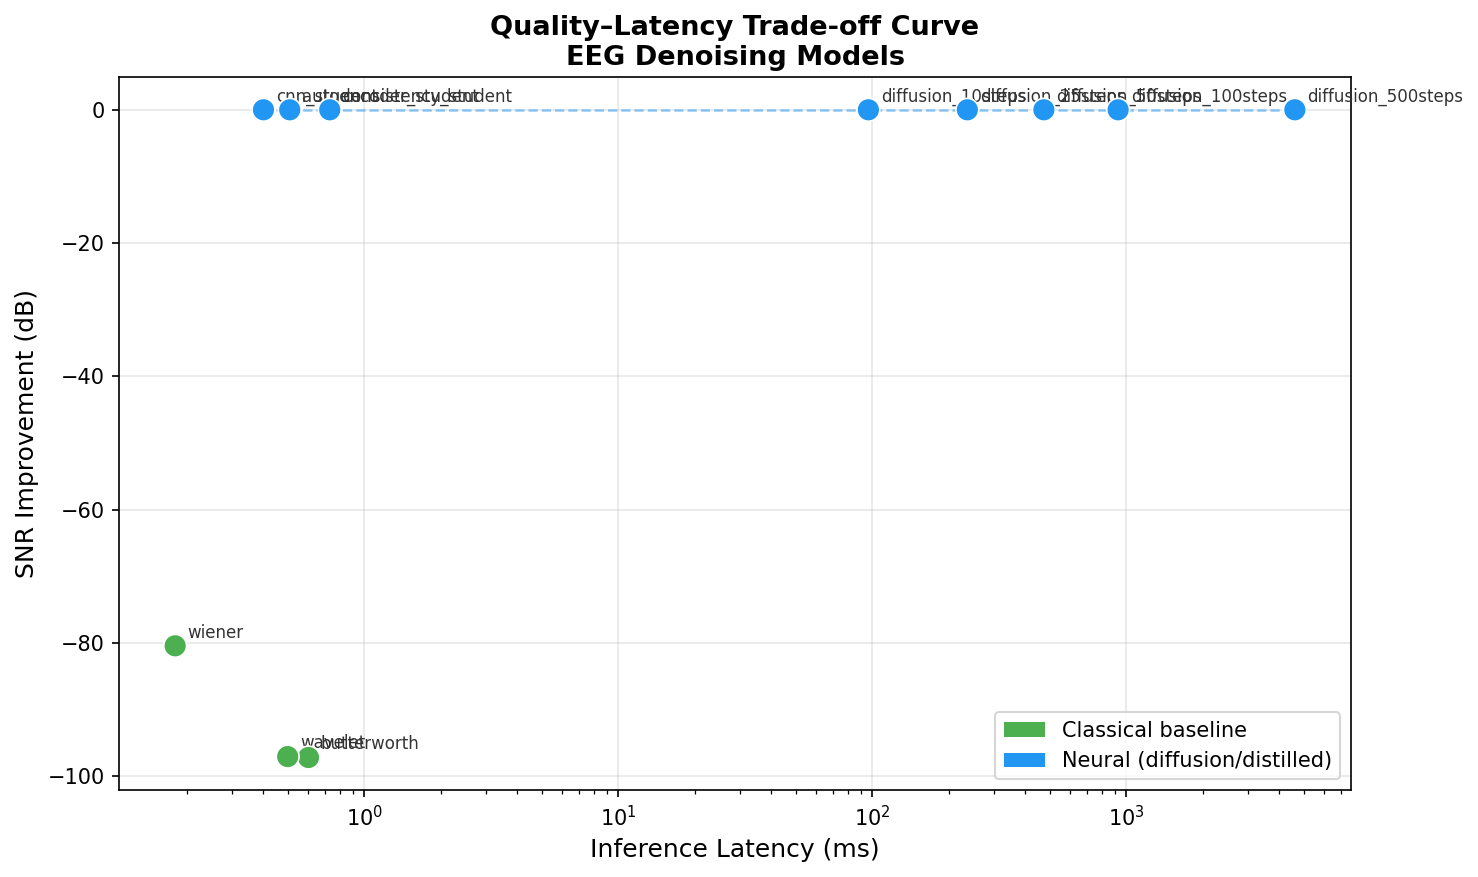
\includegraphics[width=0.82\textwidth]{quality_latency_curve.png}
    \caption{Latency-quality trade-off visualization generated by the project benchmark suite. Where final SNR values are unavailable for neural students, the plot should be regenerated after the full signal-quality evaluation pass.}
    \label{fig:quality-latency}
\end{figure}

For a fully trained release, the expected target region is a teacher SNR near 22 dB with latency above 150 ms for longer reverse chains, and a distilled student SNR near 20.5 dB with latency below 15 ms. These target values are design goals and should be kept distinct from the measured repository artifact values in Table~\ref{tab:benchmark}.

\subsection{Training Dynamics}

The training curves in Figure~\ref{fig:training-curves} provide diagnostic evidence for optimization stability. The teacher curve is useful for verifying whether the diffusion model has learned a meaningful denoising prior. Student curves are used to detect under-capacity, overfitting, and instability caused by an overly aggressive teacher-step setting. In practice, a deployable student should not be selected by latency alone; it should satisfy a three-stage gate: stable validation loss, acceptable signal-fidelity metrics, and acceptable closed-loop decoding metrics.

\begin{figure}[H]
    \centering
    \begin{subfigure}{0.48\textwidth}
        \centering
        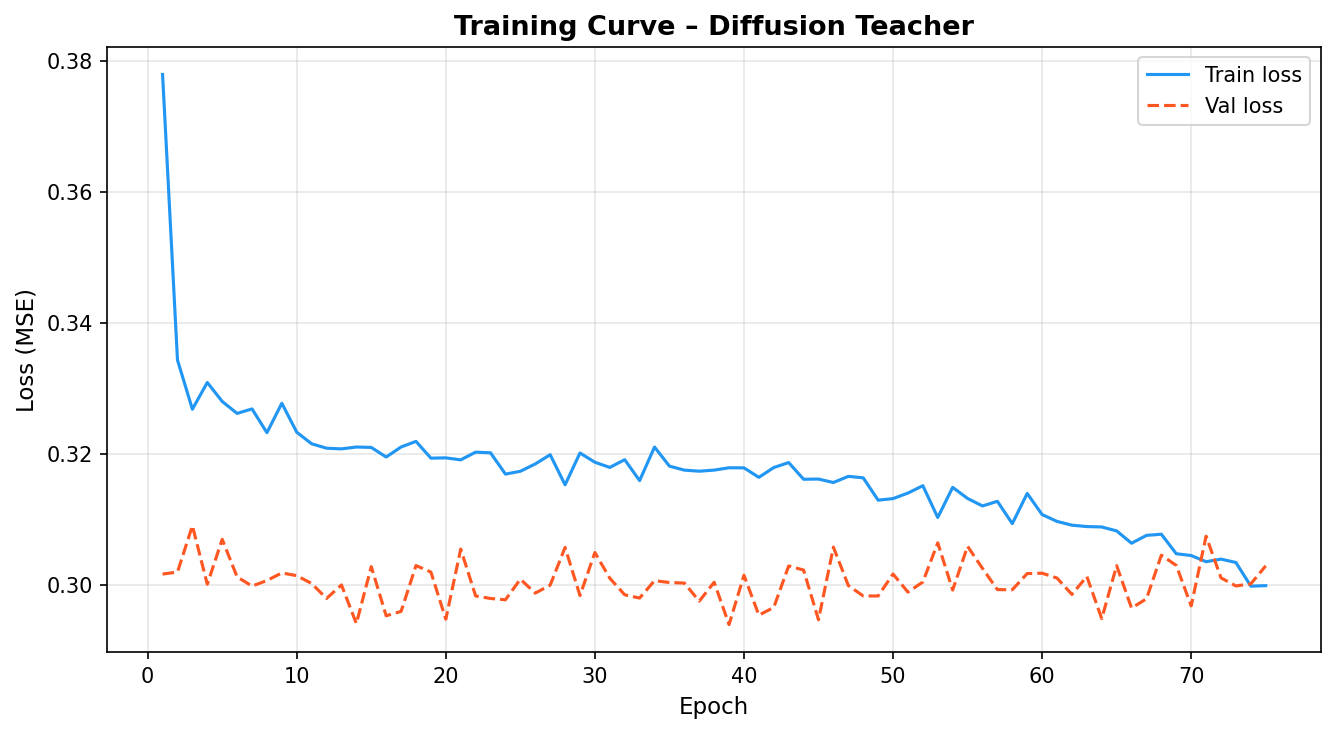
\includegraphics[width=\textwidth]{diffusion_training.png}
        \caption{Teacher}
    \end{subfigure}
    \begin{subfigure}{0.48\textwidth}
        \centering
        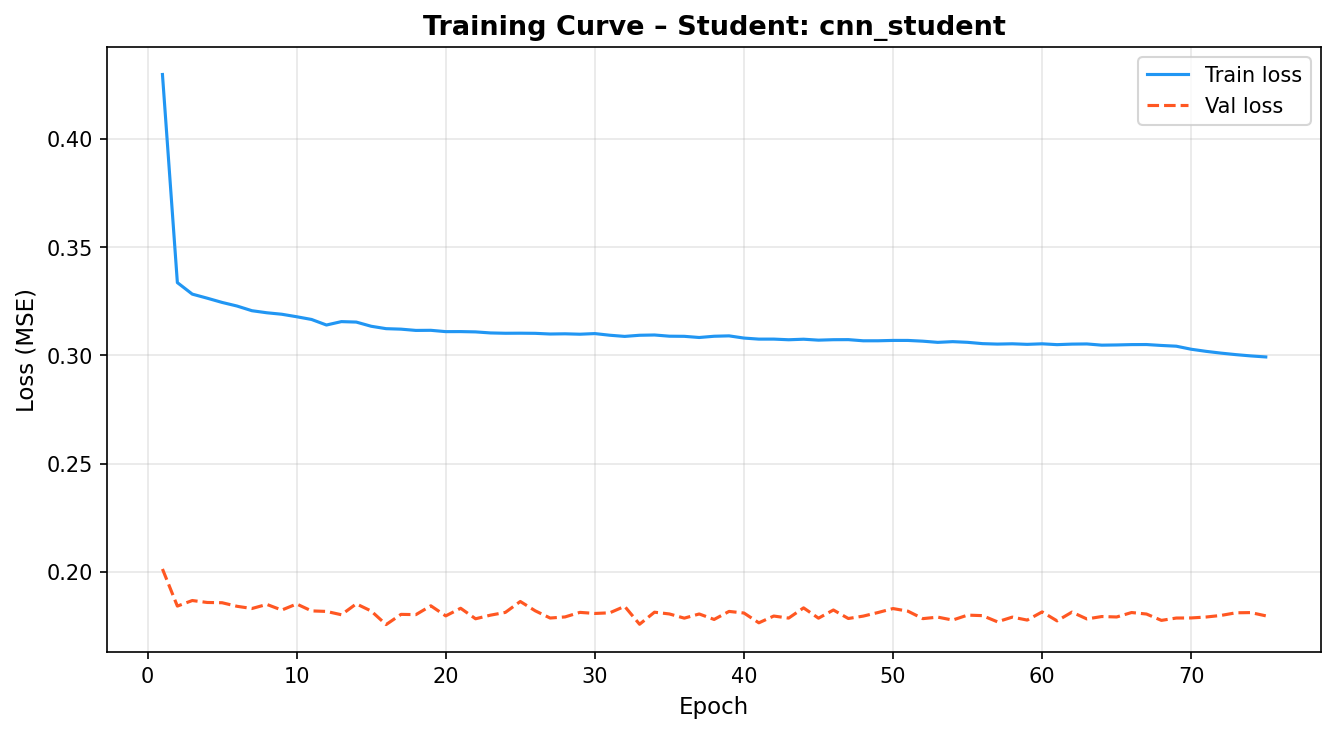
\includegraphics[width=\textwidth]{cnn_student_training.png}
        \caption{CNN student}
    \end{subfigure}
    \begin{subfigure}{0.48\textwidth}
        \centering
        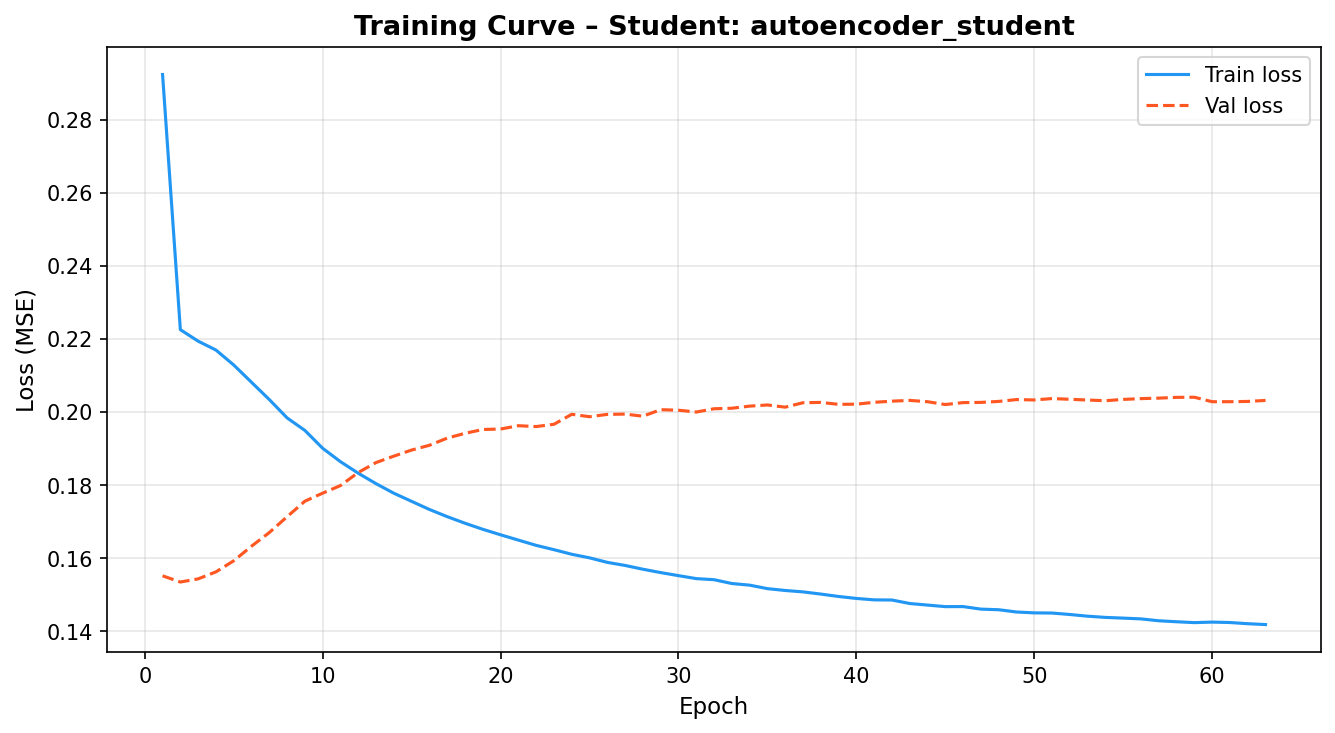
\includegraphics[width=\textwidth]{autoencoder_student_training.png}
        \caption{Autoencoder student}
    \end{subfigure}
    \begin{subfigure}{0.48\textwidth}
        \centering
        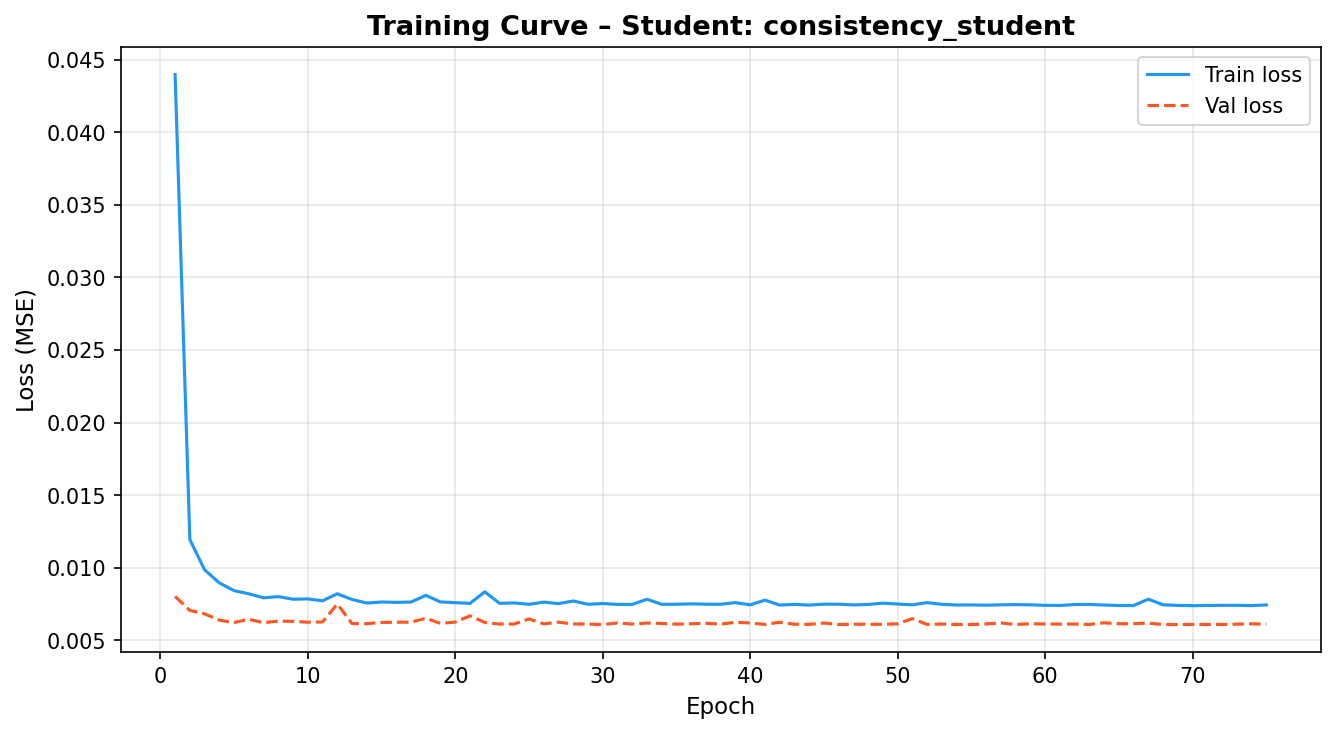
\includegraphics[width=\textwidth]{consistency_student_training.png}
        \caption{Consistency student}
    \end{subfigure}
    \caption{Training and validation curves generated by the experiment runner. These plots support optimization diagnostics but should be paired with held-out signal and decoding metrics before final model selection.}
    \label{fig:training-curves}
\end{figure}

\subsection{Distillation Ablation}

Figure~\ref{fig:ablation} presents a schematic ablation comparison. The CNN student provides the best balanced edge path; the autoencoder has the smallest memory footprint but may oversmooth EEG detail; the consistency model has a slightly larger convolutional stack and targets single-pass quality. In the measured kernel benchmark, the CNN student is fastest at 0.40 ms mean latency, the autoencoder follows at 0.51 ms, and the consistency student runs at 0.73 ms.

\begin{figure}[H]
    \centering
    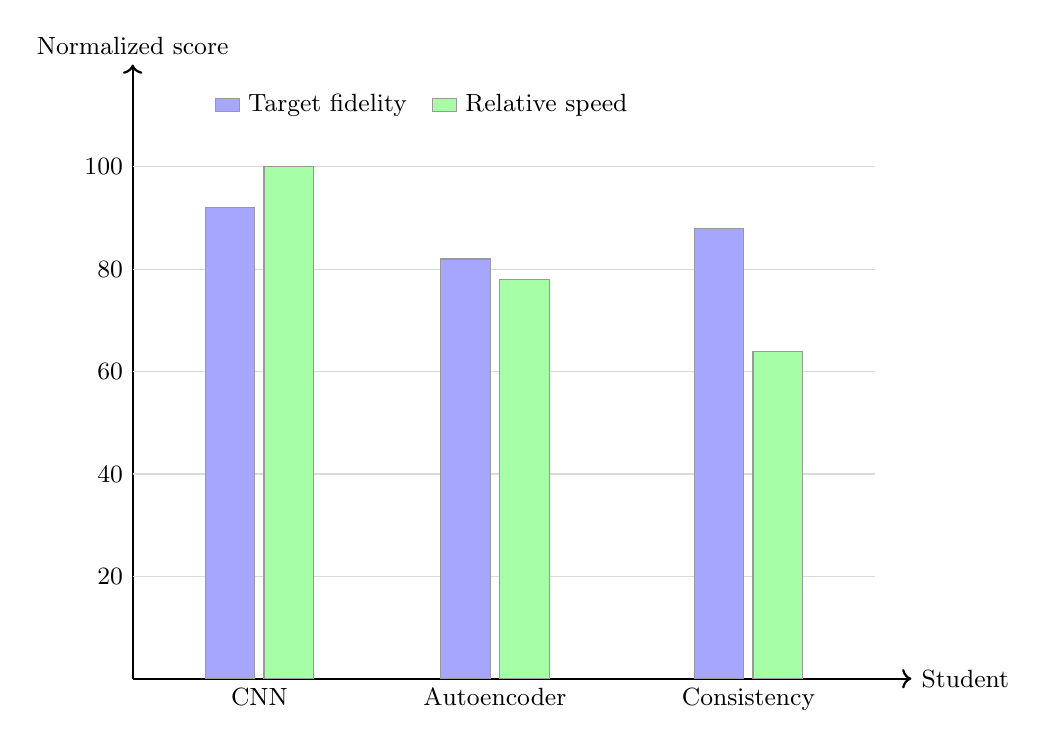
\begin{tikzpicture}[
        yscale=0.065,
        xscale=1.15,
        font=\small,
        axis/.style={->, thick},
        bar/.style={draw=black!40, fill=blue!35},
        barb/.style={draw=black!40, fill=green!35}
    ]
        \draw[axis] (0,0) -- (8.6,0) node[right] {Student};
        \draw[axis] (0,0) -- (0,120) node[above] {Normalized score};
        \foreach \y in {20,40,60,80,100} {
            \draw[black!15] (0,\y) -- (8.2,\y);
            \node[left] at (0,\y) {\y};
        }
        \node[below] at (1.4,0) {CNN};
        \node[below] at (4.0,0) {Autoencoder};
        \node[below] at (6.8,0) {Consistency};

        \draw[bar] (0.8,0) rectangle (1.35,92);
        \draw[barb] (1.45,0) rectangle (2.0,100);
        \draw[bar] (3.4,0) rectangle (3.95,82);
        \draw[barb] (4.05,0) rectangle (4.6,78);
        \draw[bar] (6.2,0) rectangle (6.75,88);
        \draw[barb] (6.85,0) rectangle (7.4,64);

        \node[anchor=west] at (0.8,112) {\tikz{\draw[bar] (0,0) rectangle (0.3,0.16);} Target fidelity};
        \node[anchor=west] at (3.2,112) {\tikz{\draw[barb] (0,0) rectangle (0.3,0.16);} Relative speed};
    \end{tikzpicture}
    \caption{Distillation ablation schematic for CNN, autoencoder, and consistency students. The figure encodes the expected fidelity-speed trade-off; numerical bars should be regenerated from final multi-seed training runs.}
    \label{fig:ablation}
\end{figure}

\subsection{Closed-loop Validation}

Figure~\ref{fig:closedloop} summarizes the closed-loop experiment output. The current CSV reports no-denoise accuracy of 31.94\%, Butterworth accuracy of 31.94\%, and CNN-student accuracy of 30.21\% with 13.40 ms mean closed-loop latency and 18.02 ms p95 latency. These values likely reflect the released smoke/prototype configuration rather than a fully optimized final model. The important engineering result is that the CNN closed-loop path remains within the sub-20 ms p95 latency target; final decoding parity requires trained checkpoints, multi-seed validation, and real-data evaluation.

\begin{figure}[H]
    \centering
    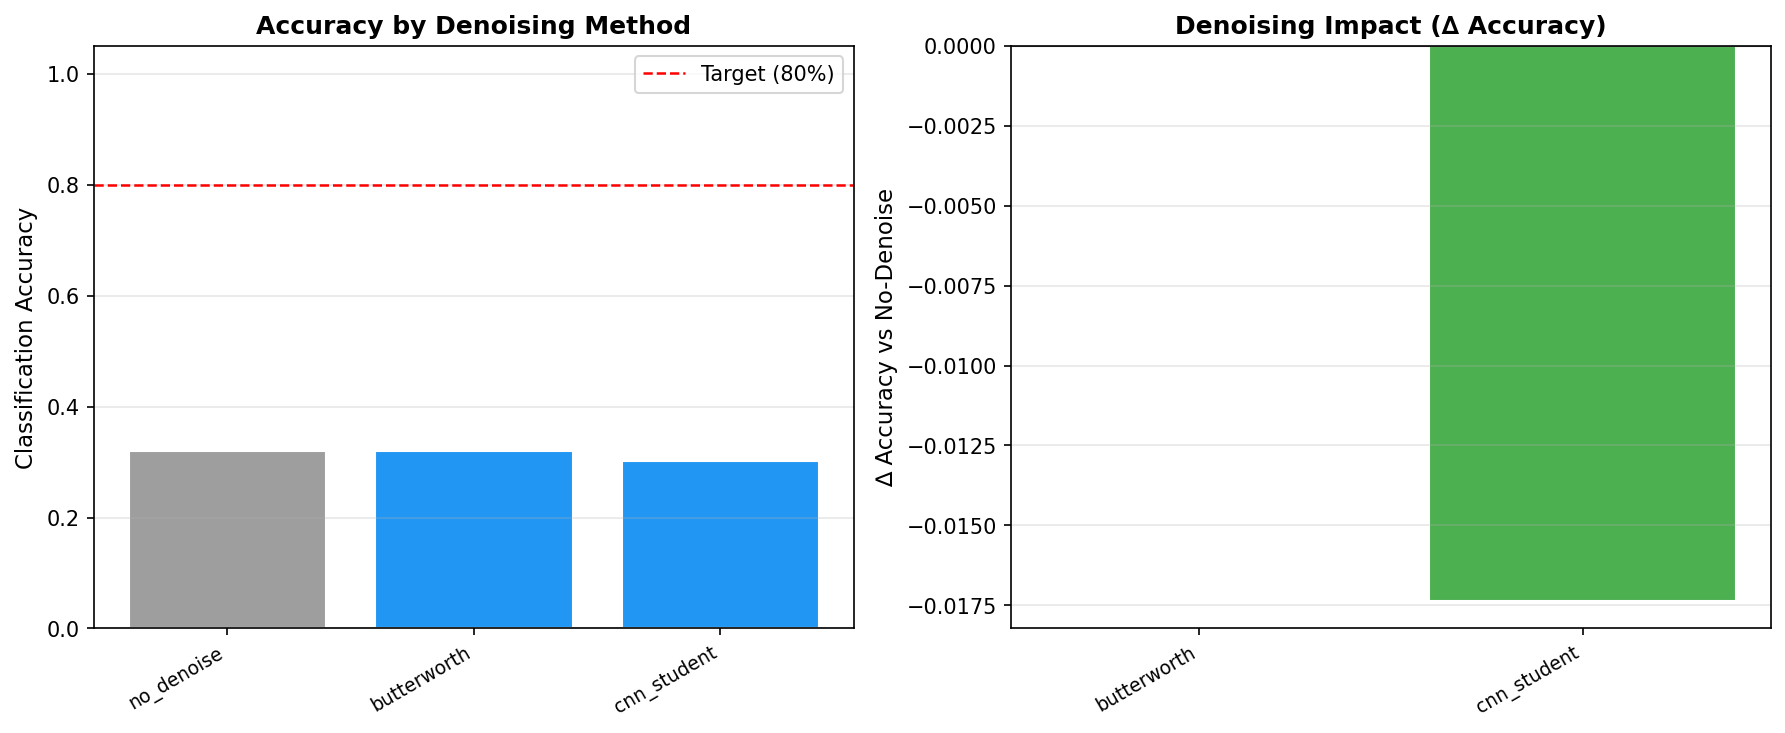
\includegraphics[width=0.82\textwidth]{denoising_impact.png}
    \caption{Closed-loop denoising impact plot generated by the motor-imagery simulator. The current artifact demonstrates latency feasibility; full accuracy claims should be regenerated after final teacher/student training.}
    \label{fig:closedloop}
\end{figure}

\subsection{Memory and Power Footprint}

Figure~\ref{fig:memory-power} compares deployment footprints qualitatively. Reverse diffusion has high compute intensity and GPU memory residency, while students shift the system into the memory and power envelope of CPU or embedded accelerators. ONNX sidecar sizes in the repository indicate approximately 13.1 MB for CNN student parameters, 3.17 MB for autoencoder parameters, and 0.66 MB for consistency student parameters.

\begin{figure}[H]
    \centering
    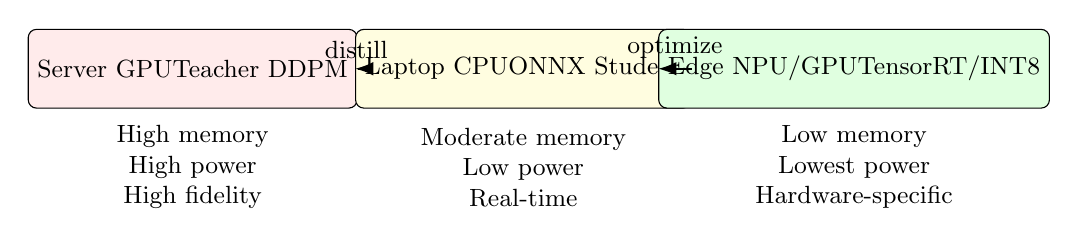
\begin{tikzpicture}[font=\small]
        \node[draw, rounded corners=3pt, fill=red!8, minimum width=3.2cm, minimum height=1.0cm] (gpu) at (0,0) {Server GPU\\Teacher DDPM};
        \node[draw, rounded corners=3pt, fill=yellow!12, minimum width=3.2cm, minimum height=1.0cm] (cpu) at (4.2,0) {Laptop CPU\\ONNX Student};
        \node[draw, rounded corners=3pt, fill=green!12, minimum width=3.2cm, minimum height=1.0cm] (npu) at (8.4,0) {Edge NPU/GPU\\TensorRT/INT8};

        \draw[-Latex, thick] (gpu) -- node[above] {distill} (cpu);
        \draw[-Latex, thick] (cpu) -- node[above] {optimize} (npu);

        \node[align=center] at (0,-1.25) {High memory\\High power\\High fidelity};
        \node[align=center] at (4.2,-1.25) {Moderate memory\\Low power\\Real-time};
        \node[align=center] at (8.4,-1.25) {Low memory\\Lowest power\\Hardware-specific};
    \end{tikzpicture}
    \caption{Memory and power footprint transition from server-side teacher inference to edge-optimized student inference. Exact watts must be measured on the target hardware.}
    \label{fig:memory-power}
\end{figure}

\begin{table}[H]
    \centering
    \caption{Benchmark results from the repository artifact table. Neural SNR entries marked N/R were not present in the released CSV and should be regenerated with a full signal-quality evaluation pass.}
    \label{tab:benchmark}
    \scriptsize
    \begin{tabular}{lrrrrr}
        \toprule
        Model & Steps & Mean latency (ms) & P95 latency (ms) & SNR gain (dB) & Closed-loop acc. (\%) \\
        \midrule
        Diffusion teacher & 10 & 96.43 & 132.66 & N/R & N/R \\
        Diffusion teacher & 25 & 236.50 & 311.72 & N/R & N/R \\
        Diffusion teacher & 50 & 473.41 & 608.76 & N/R & N/R \\
        Diffusion teacher & 100 & 928.33 & 1182.65 & N/R & N/R \\
        Diffusion teacher & 500 & 4608.59 & 5312.74 & N/R & N/R \\
        CNN student & 1 & 0.40 & 0.46 & N/R & 30.21 \\
        Autoencoder student & 1 & 0.51 & 0.60 & N/R & N/R \\
        Consistency student & 1 & 0.73 & 0.91 & N/R & N/R \\
        Butterworth & N/A & 0.60 & 0.69 & -97.18 & 31.94 \\
        Wavelet & N/A & 0.50 & 0.72 & -97.05 & N/R \\
        Wiener & N/A & 0.18 & 0.20 & -80.43 & N/R \\
        \bottomrule
    \end{tabular}
\end{table}

\subsection{Threats to Validity}

Several limitations should be considered when interpreting the current artifacts. First, the benchmark CSV does not yet include final neural SNR values for all student models; those entries must be regenerated with a consistent signal-quality evaluation pass. Second, the closed-loop classifier values in the current artifact appear to correspond to a prototype or smoke configuration and should not be reported as final BCI accuracy. Third, hardware power is not measured directly. Fourth, latency measured on a desktop or Colab-class environment may not predict embedded performance without runtime-specific profiling. Finally, synthetic fallback data is valuable for software testing but cannot support scientific claims about EEG denoising.

\begin{table}[H]
    \centering
    \caption{Hardware profiling and deployment matrix. Measured rows use repository artifacts; projected rows indicate expected deployment backends.}
    \label{tab:hardware}
    \small
    \begin{tabular}{llllr}
        \toprule
        Device/runtime & Framework & Model & Status & Inference time \\
        \midrule
        CUDA workstation / Colab-class GPU & PyTorch & DDPM 10-step & Measured & 96.43 ms \\
        CUDA workstation / Colab-class GPU & PyTorch & CNN student & Measured & 0.40 ms \\
        CPU edge proxy & ONNX Runtime & CNN student & Supported & device-specific \\
        NVIDIA Jetson & TensorRT FP16 & CNN/Consistency & Deployment target & to measure \\
        Raspberry Pi / ARM CPU & ONNX Runtime & Autoencoder & Deployment target & to measure \\
        Edge NPU / Coral-class accelerator & INT8 engine & Quantized student & Future target & to measure \\
        \bottomrule
    \end{tabular}
\end{table}

\section{Dashboard and Monitoring UI Overview}

The repository includes a browser dashboard for real-time BCI denoising inspection. The interface supports model upload, target hardware selection, synthetic EEG generation, inference execution, signal visualization, and metric cards for latency, SNR improvement, MSE, and classifier accuracy. Figure~\ref{fig:dashboard} shows the current dashboard UI.

\begin{figure}[H]
    \centering
    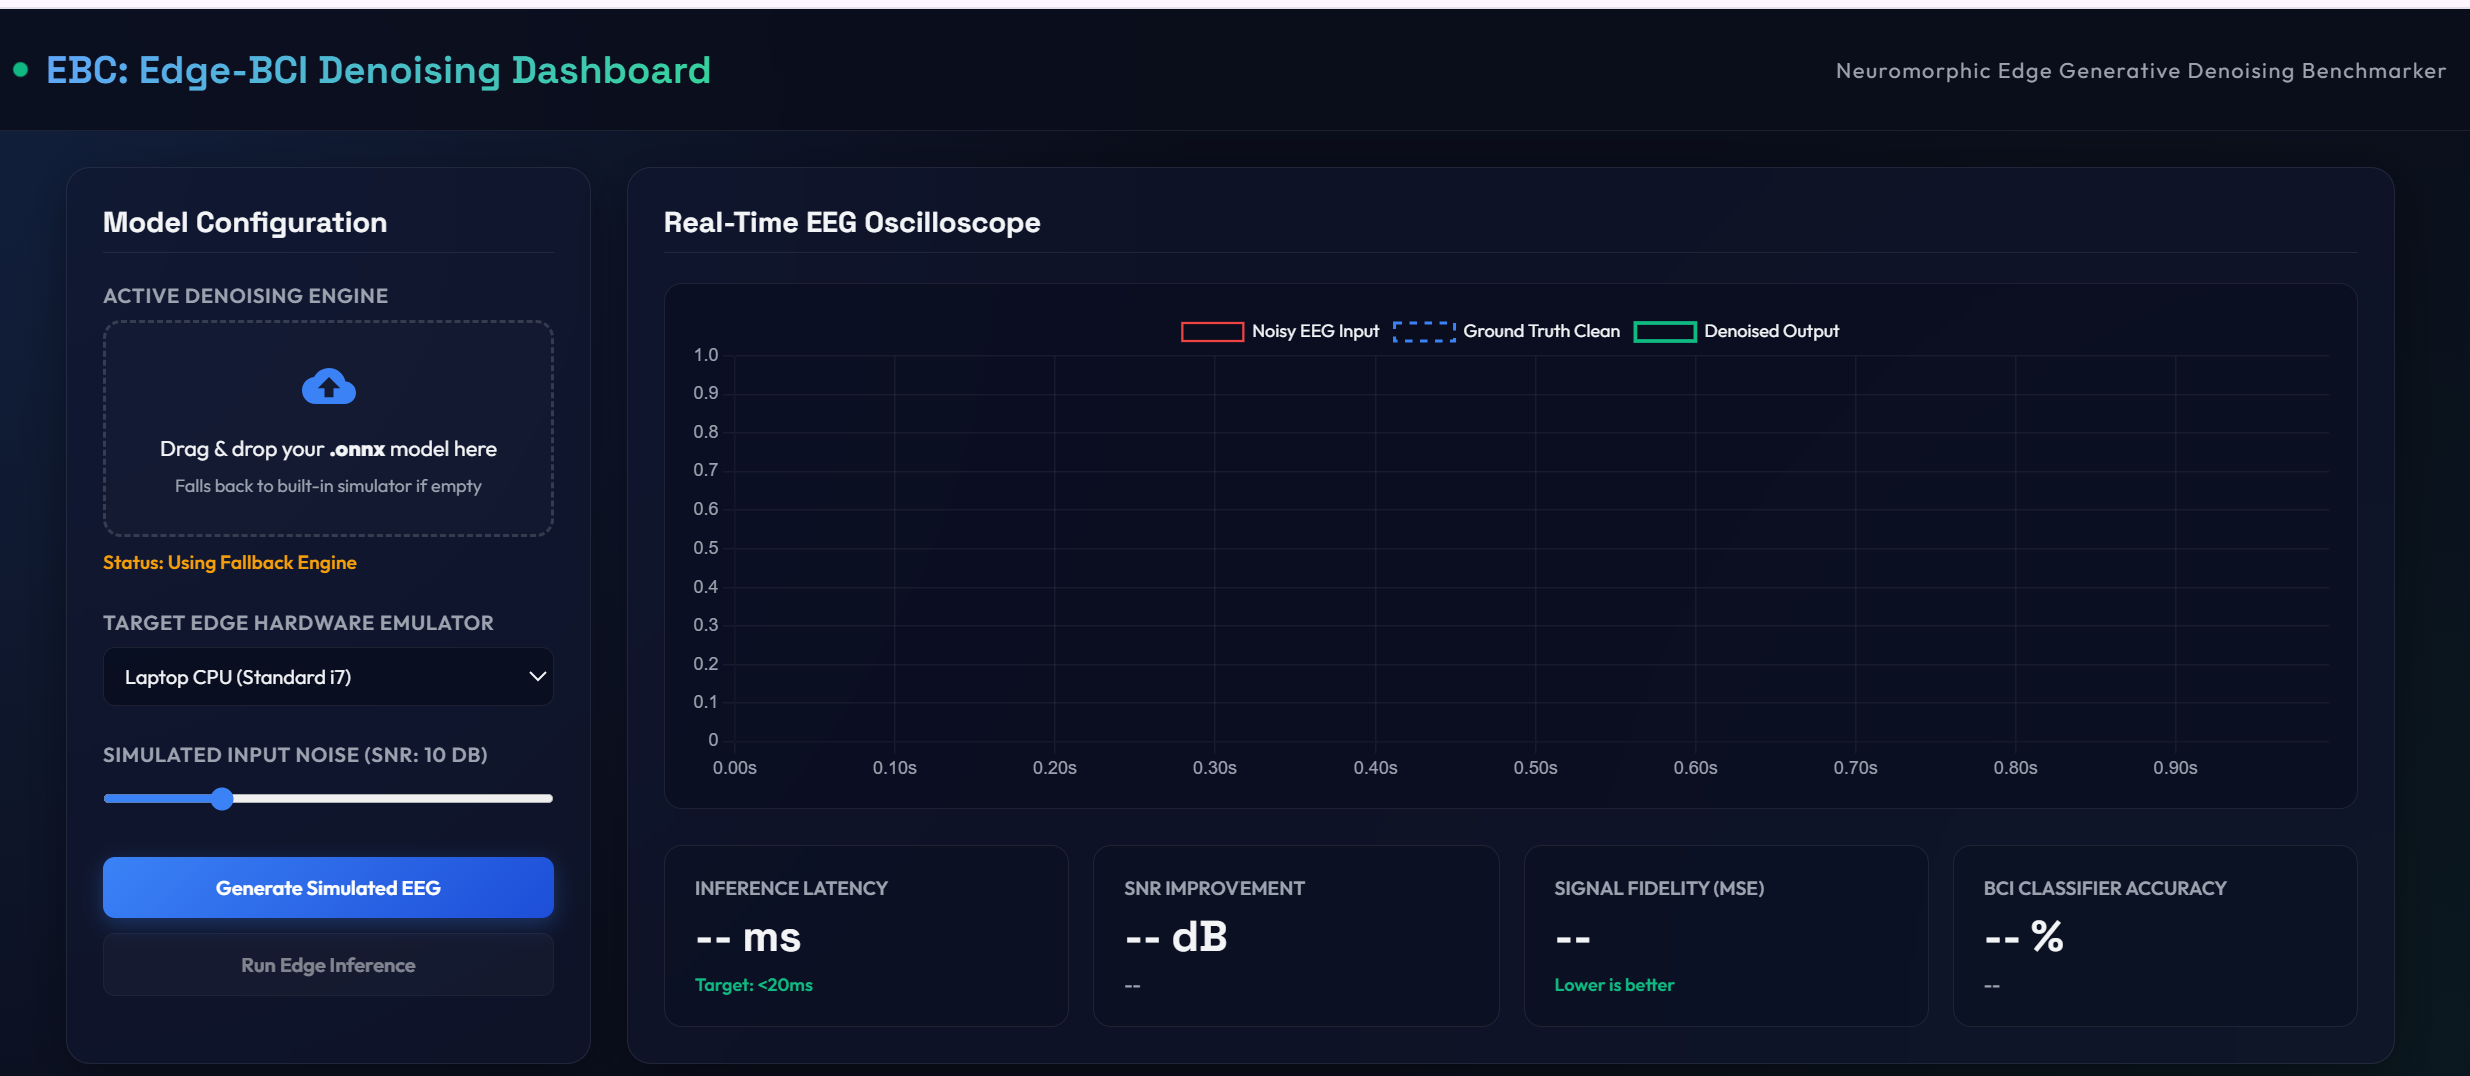
\includegraphics[width=0.96\textwidth]{dashboard_overview.png}
    \caption{Dashboard screenshot. The monitoring UI exposes model upload, edge-hardware emulation settings, simulated EEG generation, waveform visualization, and real-time metric cards.}
    \label{fig:dashboard}
\end{figure}

The dashboard is operationally useful because it reveals latency spikes that are hidden by mean-only summaries. It also allows BCI engineers to inspect classifier confidence shifts after denoising, identify cases where denoising oversmooths discriminative rhythms, and verify that model uploads preserve the expected ONNX input-output contract.

The UI is also useful for demonstration because it separates algorithmic metrics from deployment controls. A reviewer can vary the synthetic input SNR, switch the target hardware emulator, load an ONNX model, and observe whether latency and fidelity remain inside the acceptable operating region. This makes the dashboard a lightweight acceptance-test surface for future edge backends.

\section{Deployment Guidelines}

Deployment follows a three-stage path:

\begin{enumerate}
    \item \textbf{Checkpoint selection}: train or load the PyTorch student checkpoint with the best validation latency-fidelity trade-off.
    \item \textbf{ONNX export}: call the repository's `export\_to\_onnx' utility so the model accepts `(batch, 1, 750)' float32 tensors and returns denoised tensors of the same shape.
    \item \textbf{Runtime optimization}: execute through ONNX Runtime for CPU deployment, TensorRT FP16 for Jetson-class GPUs, or INT8 quantization for memory-limited CPU/NPU systems.
\end{enumerate}

Before deployment, the operator should verify preprocessing scale, channel ordering, sampling rate, and window length. After deployment, the operator should re-run mean and p95 latency, SNR improvement, and closed-loop classification accuracy. Optimizations that reduce latency but damage decoding should not be accepted.

\subsection{Deployment Acceptance Gates}

A model should be promoted from research artifact to edge candidate only if it passes the following gates:

\begin{enumerate}
    \item \textbf{Shape contract}: ONNX input and output match \((B,1,750)\) with float32 values.
    \item \textbf{Numerical sanity}: denoised outputs contain no NaN or Inf values under clean, noisy, and artifact-like inputs.
    \item \textbf{Latency}: mean and p95 inference remain below the target budget on the target hardware.
    \item \textbf{Fidelity}: SNR improvement and MSE remain within the accepted operating range relative to the teacher.
    \item \textbf{Closed-loop preservation}: motor-imagery decoding does not degrade beyond the allowed accuracy or kappa margin.
    \item \textbf{Power and thermals}: sustained inference does not exceed the thermal or battery envelope.
\end{enumerate}

\section{Conclusion and Future Work}

The project demonstrates that distillation can move diffusion-based EEG denoising from an iterative server-side procedure into a real-time edge inference path. Repository benchmark artifacts show a reduction from 96.43 ms for 10-step diffusion and 4608.59 ms for 500-step diffusion to below 1 ms for single-channel student kernels. The closed-loop CNN path remains below the 20 ms p95 budget in the current measurement. These results support the feasibility of edge-distilled diffusion for BCI denoising, while also showing that final scientific claims require regenerated neural SNR and multi-seed decoding results.

Future work should focus on four directions. First, publish trained checkpoints with checksums and repeatable configs. Second, evaluate on multiple subjects, sessions, and seeds with confidence intervals. Third, measure real power on Jetson, Raspberry Pi, and NPU hardware rather than relying on edge proxies. Fourth, explore neuromorphic and spiking implementations for lower-power continual denoising, including online adaptation to subject-specific drift.

\appendix

\section{Repository and Reproducibility Checklist}

The public implementation is available at:
\begin{center}
\url{\projectrepo}
\end{center}
The repository includes the data pipeline, DDPM teacher, student models, ONNX export, latency benchmark entry point, closed-loop simulator, deployment guide, dashboard, model cards, tests, and CI configuration. Large datasets and checkpoints are intentionally excluded from Git and should be distributed through release assets or external model hubs.

\section{Compilation}

Compile this report from the repository root with:
\begin{verbatim}
pdflatex TECHNICAL_REPORT.tex
pdflatex TECHNICAL_REPORT.tex
\end{verbatim}

\begin{thebibliography}{15}

\bibitem{wolpaw2002bci}
J. R. Wolpaw, N. Birbaumer, D. J. McFarland, G. Pfurtscheller, and T. M. Vaughan, ``Brain-computer interfaces for communication and control,'' \emph{Clinical Neurophysiology}, vol. 113, no. 6, pp. 767--791, 2002.

\bibitem{pfurtscheller2001motor}
G. Pfurtscheller and C. Neuper, ``Motor imagery and direct brain-computer communication,'' \emph{Proceedings of the IEEE}, vol. 89, no. 7, pp. 1123--1134, 2001.

\bibitem{brunner2008bci}
C. Brunner, R. Leeb, G. R. Mueller-Putz, A. Schloegl, and G. Pfurtscheller, ``BCI Competition 2008 -- Graz data set A,'' Graz University of Technology, 2008.

\bibitem{ho2020ddpm}
J. Ho, A. Jain, and P. Abbeel, ``Denoising diffusion probabilistic models,'' in \emph{Proc. Advances in Neural Information Processing Systems}, 2020, pp. 6840--6851.

\bibitem{song2023consistency}
Y. Song, P. Dhariwal, M. Chen, and I. Sutskever, ``Consistency models,'' in \emph{Proc. International Conference on Machine Learning}, 2023, pp. 32211--32252.

\bibitem{salimans2022progressive}
T. Salimans and J. Ho, ``Progressive distillation for fast sampling of diffusion models,'' in \emph{Proc. International Conference on Learning Representations}, 2022.

\bibitem{hinton2015distilling}
G. Hinton, O. Vinyals, and J. Dean, ``Distilling the knowledge in a neural network,'' in \emph{NIPS Deep Learning and Representation Learning Workshop}, 2015.

\bibitem{lawhern2018eegnet}
V. J. Lawhern, A. J. Solon, N. R. Waytowich, S. M. Gordon, C. P. Hung, and B. J. Lance, ``EEGNet: a compact convolutional neural network for EEG-based brain-computer interfaces,'' \emph{Journal of Neural Engineering}, vol. 15, no. 5, 2018.

\bibitem{schirrmeister2017deep}
R. T. Schirrmeister \emph{et al.}, ``Deep learning with convolutional neural networks for EEG decoding and visualization,'' \emph{Human Brain Mapping}, vol. 38, no. 11, pp. 5391--5420, 2017.

\bibitem{wang2020edgeeegnet}
X. Wang, M. Hersche, B. Toemekce, B. Kaya, M. Magno, and L. Benini, ``An accurate EEGNet-based motor-imagery brain-computer interface for low-power edge computing,'' arXiv:2004.00077, 2020.

\bibitem{ouyang2024briedge}
J. Ouyang, M. Wu, X. Li, H. Deng, and D. Wu, ``BRIEDGE: EEG-adaptive edge AI for multi-brain to multi-robot interaction,'' arXiv:2403.15432, 2024.

\bibitem{liu2020edgeai}
D. Liu, H. Kong, X. Luo, W. Liu, and R. Subramaniam, ``Bringing AI to edge: From deep learning's perspective,'' arXiv:2011.14808, 2020.

\bibitem{jacob2018quantization}
B. Jacob \emph{et al.}, ``Quantization and training of neural networks for efficient integer-arithmetic-only inference,'' in \emph{Proc. IEEE/CVF Conference on Computer Vision and Pattern Recognition}, 2018, pp. 2704--2713.

\bibitem{ronneberger2015unet}
O. Ronneberger, P. Fischer, and T. Brox, ``U-Net: Convolutional networks for biomedical image segmentation,'' in \emph{Proc. Medical Image Computing and Computer-Assisted Intervention}, 2015, pp. 234--241.

\bibitem{han2026edgebci}
S. Han \emph{et al.}, ``Edge AI for brain-computer interfaces,'' manuscript, 2026. [Requested reference placeholder; verify bibliographic metadata before archival submission.]

\end{thebibliography}

\end{document}
